\chapter{Literature Review}
This chapter introduces some existing document management system.
Section \ref{dms-features} gives lists of required features of \dms.
Section \ref{relate-works} explores some existing document management applications.

\section{Integrated features} \label{dms-features}
Document management is the process of applying policies and rules to how documents are created, persisted, and expired within an organization.
We analysed each service based on the following features.

\begin{description}
\item[Access Control] \hfill \\
This feature controls how much user can interact with the document.
The system should use role-based access control to authorize the user because \gls{ic} classify employees by their responsibilities.
A role-based access control defines what operation user can perform based on their roles.

\item[Archiving and Retention] \hfill \\
How the system stores documents on a permanent storage.
How the system search and retrieve files.
This feature manage the files and how to access them.

\item[Collaboration] \hfill \\
This feature enables users to cooperate with other individuals on the same document. 

\item[Document Assembly] \hfill \\
This feature assists user to create a digital document.
It provides the document with pre-existing text called a template when the user creates a new document.

\item[Version Control] \hfill \\
Version control is the management of changes to documents.
It stores changes' history for later recovery.
In this case, the system has to have a periodic document backup when user is editing a document.
Lastly, user should be able to create new revision of document when they ready to publish the document.

\item[Form Management] \hfill \\
This feature let user creates and manages document forms.
The system treats form as another type of document.
The difference is user can fill in the blank fields provided in the document.

\item[Document Searching Service] \hfill \\
When user request a document, the system will look in its storage based on given keywords.
User does not have to look within the storage by oneself.
The system provides user with various searching criteria for user to get what they need.
\end{description}

\section{Related Works} \label{relate-works}
We pick 9 existing document management applications to investigate.
Each application has its interesting functionalities and characteristics.
We review them based on 7 characteristic features as stated above.

\begin{description}
\item[Alfresco One] \hfill \\
Alfresco One allows organizations to manage any type of content from small office documents, photographs, to large video files.
The system allows users to choose how to access their content --- via the Web, desktop or email --- while the server enforces access controls and security.
\begin{figure}[h]
	\centering
	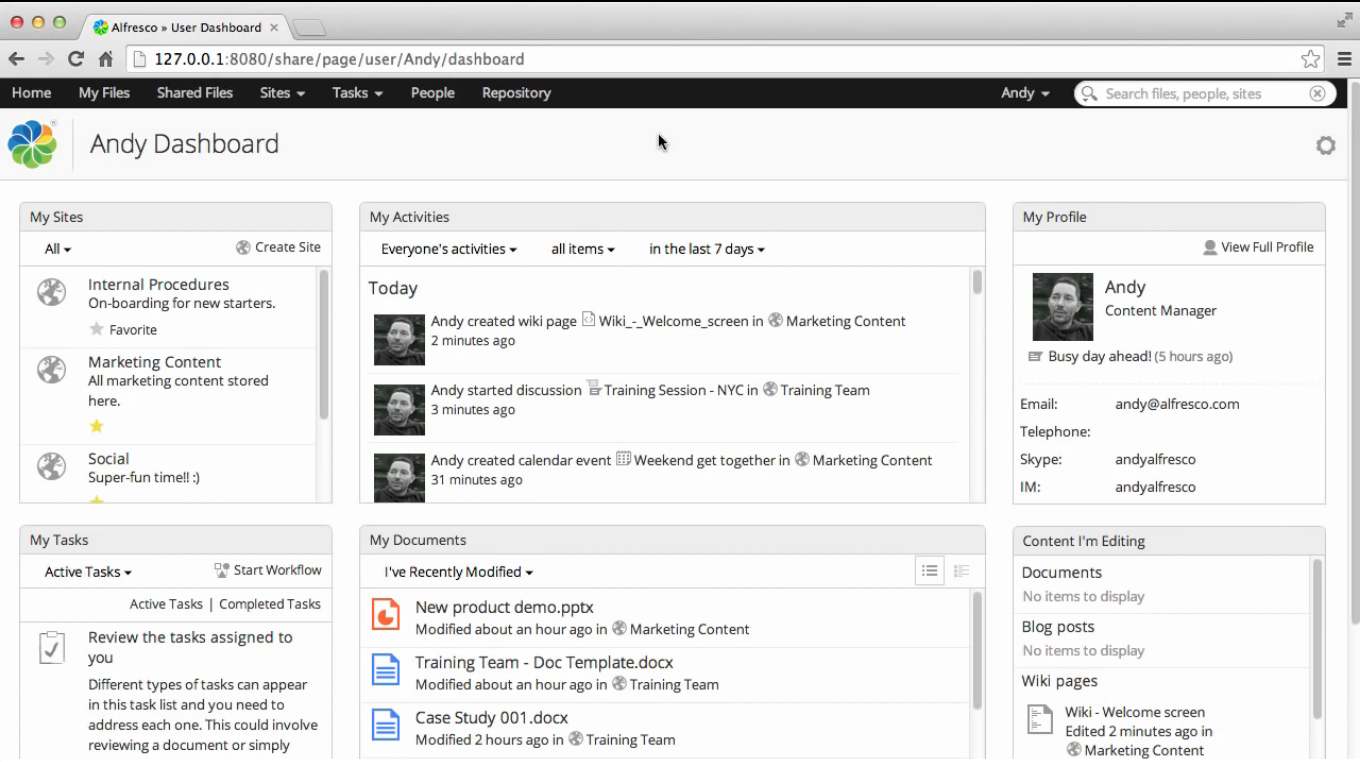
\includegraphics[scale=0.4]{res/literature/screenshot_alfresco}
	\caption{A screenshot of Alfresco One (Community Edition) 5.0.0d \citefigure{alfresco}}
\end{figure}

\item[Dokmee] \hfill \\
Dokmee has multiple editions targeted at companies of all sizes.
It can run in a Windows-based Intranet network, as a Web-hosted system or as an individual software on a personal computer.
User can organize files into folders and can store unlimited number of files.
\begin{figure}[h]
	\centering
	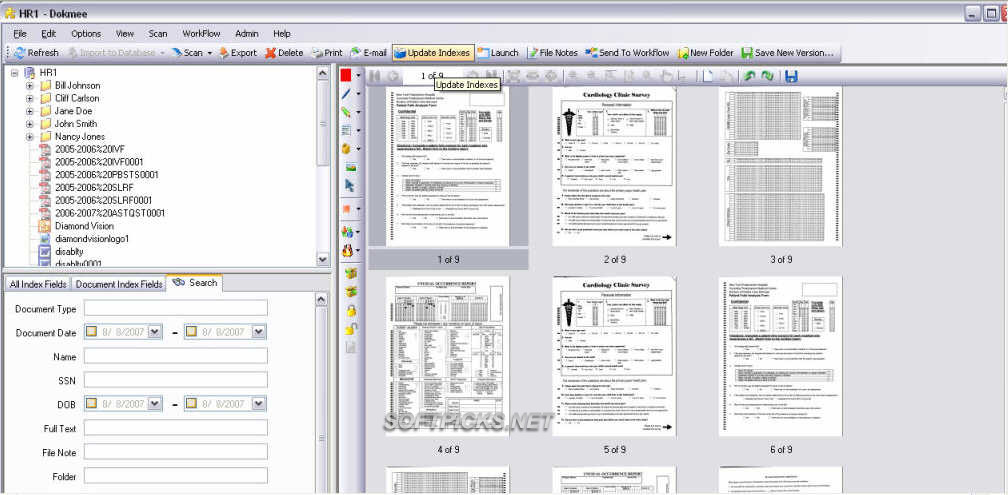
\includegraphics[scale=0.55]{res/literature/screenshot_dokmee}
	\caption{A screenshot of Dokmee 3.0.2.4 \citefigure{dokmee}}
\end{figure}

\item[Asite Document Manager] \hfill \\
Asite Document Manager provides an organization with a centralize storage with folder-like structure.
They claim that doing so saves user's time and effort of each party managing their own filing system.

\item[Eclipse Document Managment] \hfill \\
This program, developed by docSTAR, offers solution for storing and scanning electronic document files.
User can grant access to documents based on user permission.
It has a centralized storage accessible from other locations.
It searches documents by text, field, annotation, and name with auto-complete feature.
The program also claims that it can locate documents that have a similar pronunciation too.
\begin{figure}[h]
	\centering
	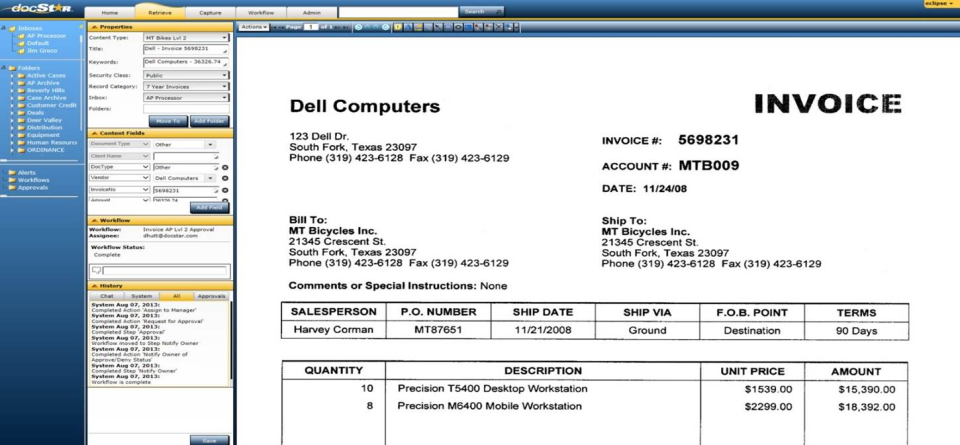
\includegraphics[scale=0.8]{res/literature/screenshot_docstar}
	\caption{A screenshot of Eclipse Document Managment 3.1 \citefigure{docstar}}
\end{figure}

\item[eFileCabinet] \hfill \\
eFileCabinet hosts documents on their cloud server.
It searches document by filename and tags.
The program saves search history every time user perform a search for auto completion.
It can look for word and phrases inside a document.
User can sends document directly to eFileCabinet from Windows File Explorer or Microsoft Office Products (Add-ons).
\begin{figure}[h]
	\centering
	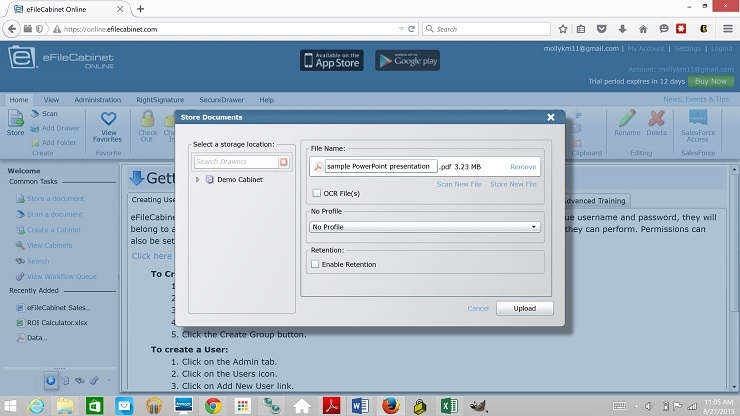
\includegraphics[scale=0.7]{res/literature/screenshot_efilecabinet}
	\caption{A screenshot of eFileCabinet 2014 \citefigure{efilecabinet}}
\end{figure}

\item[Contentverse] \hfill \\
Contentverse has file naming and storing similar to cabinet and folder structure, indexed for immediate full-text search and retrieval.
The program track every changes -- every version of any file available for reference.
The program allows user to assign permission to users based on their specific roles.
\begin{figure}[h]
	\centering
	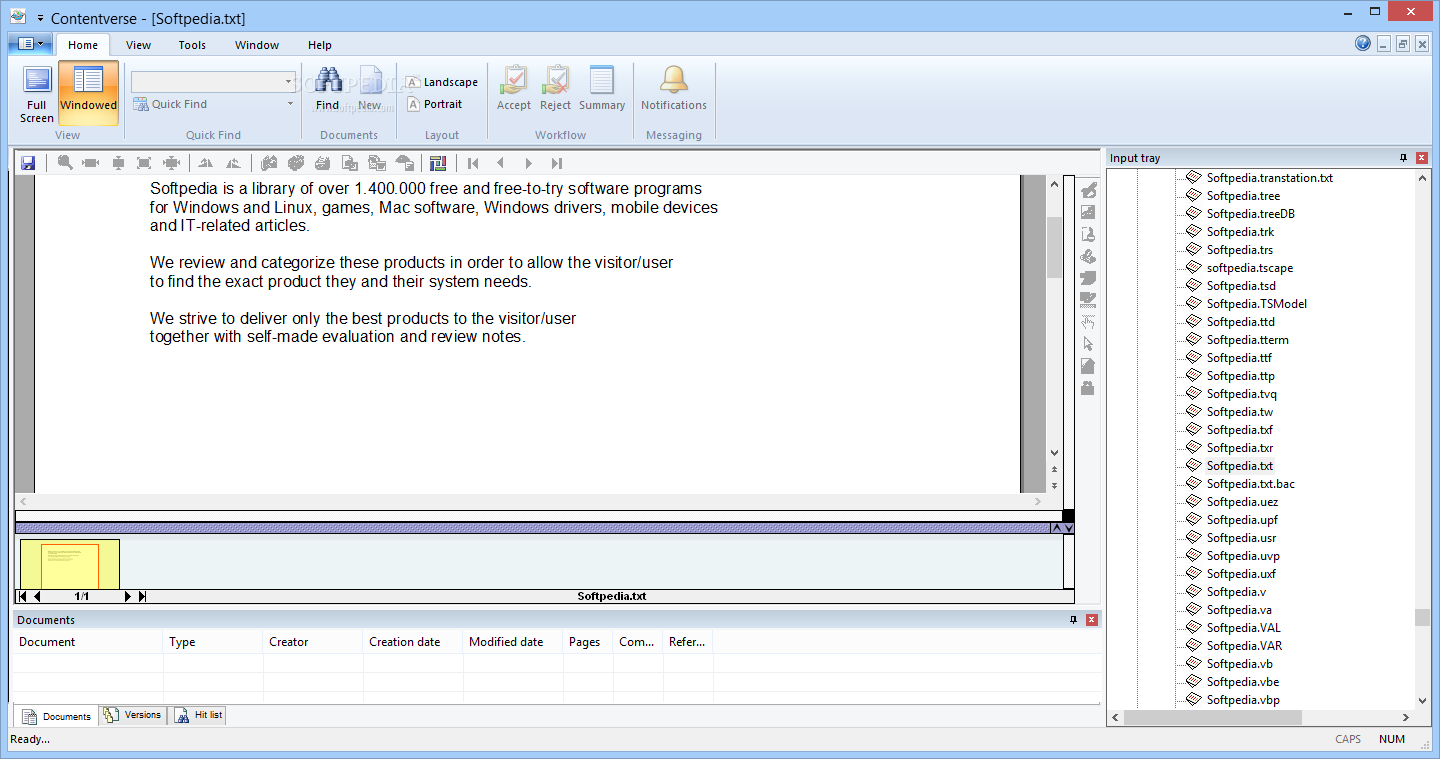
\includegraphics[scale=0.35]{res/literature/screenshot_contentverse}
	\caption{A screenshot of Contentverse 8.0 \citefigure{contentverse}}
\end{figure}

\item[SmartFile] \hfill \\
SmartFile is a file management solution that enables everyone to securely share, manage and control files both offline and online.
SmartFile offers \gls{OCR} search.
User can find content within their documents.
The program narrows search result by let user specify date interval and file size interval.
User can view PDF, JPG, PNG, GIF, and other image formats with its own viewer.
The characteristics of this program is its permanent activity logs storage.
An activity log contain file's access information, who access the file, what user did to the file.
These logs are kept in the program permanently.

\item[isoTracker Document Control] \hfill \\
The software encrypts documents and stores safely in folders.
User can set access permission on files or folders themselves.
The program search documents by metadata and tags.
Documents can be reviewed, commented on and modified. 
The software also features a complete usage log for each document.

\item[Zoho Docs] \hfill \\
Zoho Docs is a document management system on a cloud server.
User can access the file anywhere on their smart phone device.
The software encourages real-time collaboration among other team members.
The program also has its own tools for creating word documents, spreadsheets, and presentations.
Search feature of this program can search by filename only.
It can not search for contents within the file.
Zoho Docs has a predefined folders separate by categories such as accounts, sales, and marketing.
User can create a multi-level folder structure to organize their files.
\begin{figure}[h]
	\centering
	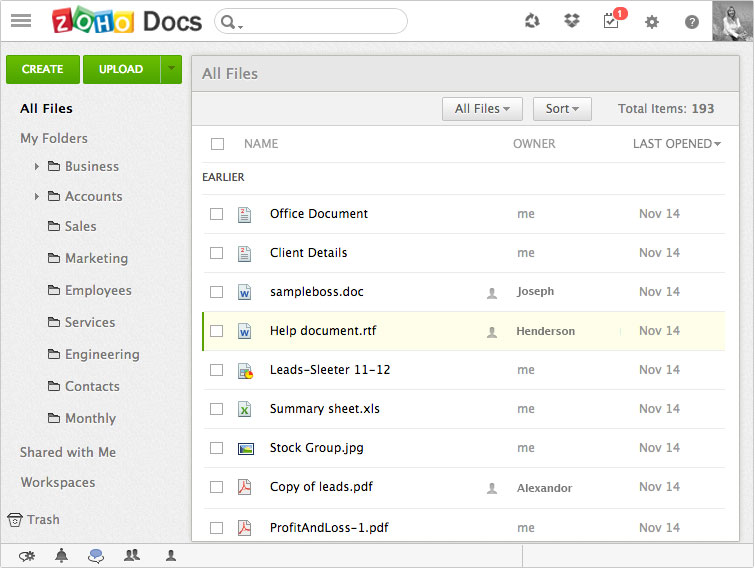
\includegraphics[scale=0.55]{res/literature/screenshot_zoho}
	\caption{A screenshot of Zoho Docs \citefigure{zoho-doc}}
\end{figure}
\end{description}

Table \ref{tbl:deploy-sum} shows a comparison application platform available.
Table \ref{tbl:feature-sum} shows a comparison of features that we interested.
The symbol \enquote*{X} indicates a yes.
Otherwise, table will show \enquote*{/} symbol indicates a no.

\clearpage

\begin{table}
	\centering
	\pgfplotstabletypeset[
    col sep=comma,
    string type,
    columns/deployment/.style={
    	column name=Deployment,
    	column type={|L{3cm}|}
    	},
    columns/reqProg/.style={
       	column name=Require a program to be installed on a computer,
       	column type={C{4cm}|}
    },
    columns/hasMblApp/.style={
    	column name=Has mobile application,
    	column type={C{2cm}|}
    },
    columns/webAccess/.style={
    	column name=Access via a web browser,
    	column type={C{2cm}|}
    },        
    every head row/.style={before row=\hline,after row=\hline},
    every last row/.style={after row=\hline},
    ]{res/app-deploy-summary-all.csv}
    
    \caption{The comparison of all reviewed program by their deployment}
    \label{tbl:deploy-sum}
\end{table}

\begin{table}
	\centering
	\pgfplotstabletypeset[
	col sep=comma,
	string type,
	columns/feature/.style={
		column name=Feature,
		column type={|L{2cm}|}
	},
	columns/accessCtrl/.style={
		column name=Access Controls,
		column type={C{1.4cm}|}
	},
	columns/achiveRetent/.style={
		column name=Archiving \& Retention ,
		column type={C{1.5cm}|}
	},
	columns/collab/.style={
		column name=Collaboration,
		column type={C{1.5cm}|}
	},
	columns/docAssem/.style={
		column name=Document Assembly,
		column type={C{1.7cm}|}
	},  
	columns/formManage/.style={
		column name=Form Management,
		column type={C{1.8cm}|}
	},	      
	columns/txtSearch/.style={
		column name=Document Searching Service,
		column type={C{1.5cm}|}
	},  
	columns/verCtrl/.style={
		column name=Version Control,
		column type={C{1.5cm}|}
	},  	      		        
	every head row/.style={before row=\hline,after row=\hline},
	every last row/.style={after row=\hline},
	]{res/app-feature-summary-all.csv}
	
	\caption{The comparison of all reviewed program and their features}
	\label{tbl:feature-sum}
\end{table}

